%--------------------------------------------------------------------------------------------------
\section{Preliminaries} \label{Preliminaries} 
%--------------------------------------------------------------------------------------------------

Deliverable 3.1 State of the art of inference in hybrid and dynamic models \cite{Deliverable 3.1}.

Variational inference  \cite{Jordan1999,Attias2000}

conjugate-exponential families \cite{Attias2000,Beal2003,Bishop2005}

An overview of the data structures implemented in the AMIDST toolbox is illustrated in Figure \ref{Figure:ToolboxDataStructures}. These data structures basically define the main components that will be used for implementing the AMIDST learning and inference algorithms. As we previously mentioned, in the AMIDST toolbox, we focus on two specific instantiations of PGMs, namely, a static Bayesian network (\comp{BN} component) and a two time-slice dynamic Bayesian network (\comp{2T-DBN} component). This is also directly reflected in the component structure.

\vspace{-0.1in}

\begin{figure}[ht!]
\begin{center}
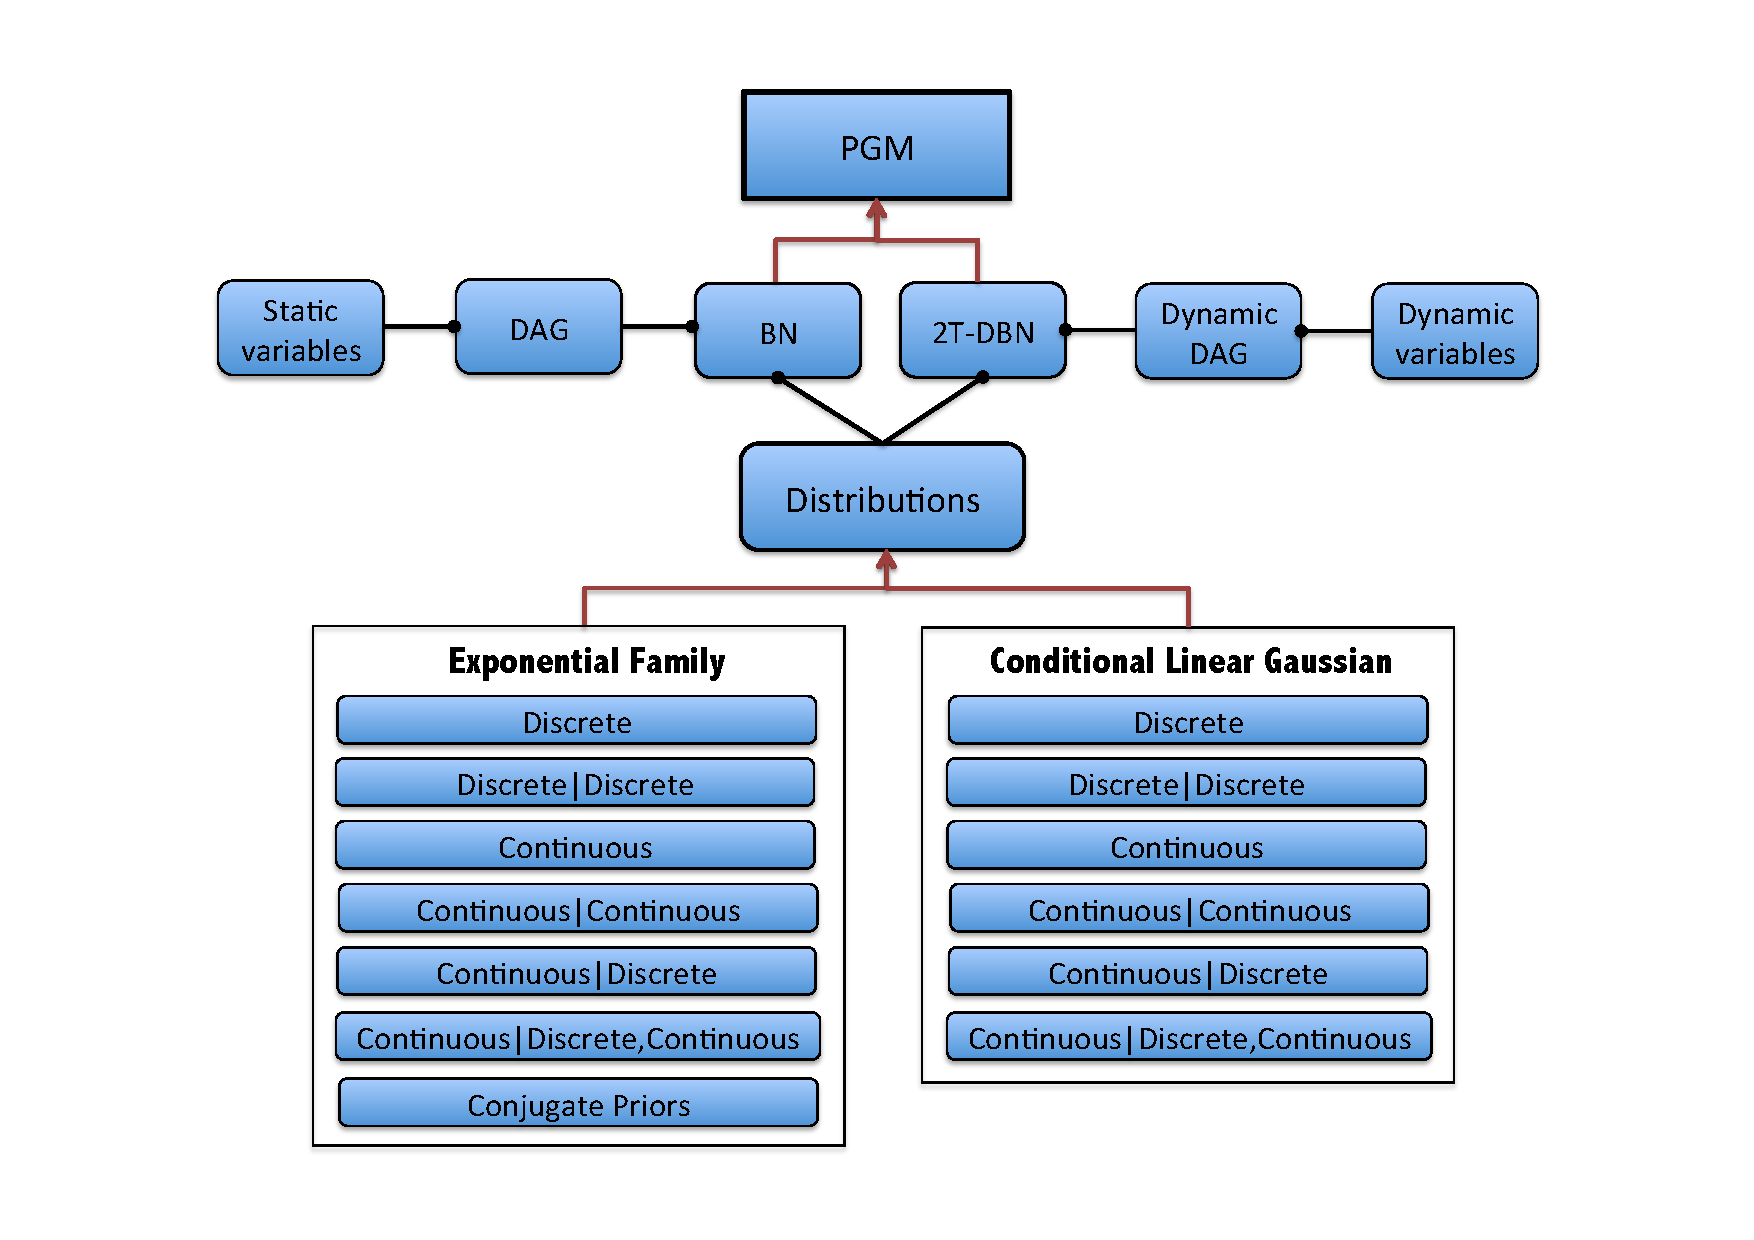
\includegraphics[width=\linewidth]{./figures/DataStructure}
\vspace{-0.5in}
\caption{\label{Figure:ToolboxDataStructures} Illustration of AMIDST toolbox data structure components. Nomenclature: The boxes in the
      figure represent software components (sets, possibly singletons, of classes), a rounded-arc going from $X$ to $Y$ indicates that $Y$ 'uses/references' $X$, and an arc with an arrow from $X$ to $Y$ implies inheritance.}
\end{center}
\end{figure}